%!TEX root = main.tex
\afterpage{\blankpage}
\newpage
\chapter{Experimentálne overenie}
\label{sec:experiment}

Navrhnutú metódu vytvárania personalizovaných informačných bulletinov sme sa rozhodli overiť prostredníctvom
nekontrolovaného online experimentu. Väčšina prác venujúcich sa odporúčaniu v doméne CQA systémov overuje
svoje hypotézy v offline experimentoch na kontrolovaných vzorkách dát. Pre účely realistického overenia našej metódy, hlavne
z pohľadu faktorov špecifických pre informačné bulletiny, však overovanie v offline experimente nie je dostačujúce.
Online nekontrolované experimenty samozrejme vyžadujú oveľa viac námahy a ich výsledky nie sú garantované, no v prípade,
že je takýto experiment úspešný, má oveľa väčší potenciál priniesť relevantné výsledky.

Experiment sme vykonávali na používateľoch z komunity Stack Overflow platformy Stack Exchange.
Komunitu Stack Overflow sme pre náš experiment zvolili z viacerých dôvodov, hlavne však preto,
že sa jedná o jednoznačne najaktívnejšiu komunitu z celej platformy, v ktorej bol najväčší potenciál získať čo najviac
používateľov do nášho experimentu. Okrem toho zohrával úlohu v rozhodovaní aj fakt, že táto komunita sa venuje doménovej
oblasti, v ktorej máme určité vedomosti, čo nám umožňilo jednoduchšie odhadnúť úroveň relevancie odporúčaného obsahu.

Do experimentu sa mohli prihlásiť všetci používatelia, ktorí majú konto na portáli Stack Overflow, prostredníctvom
registračného formuláru systému StackLetter. Celkovo sa nám podarilo získať pomerne diverznú vzorku používateľov,
medzi ktorými boli prítomní okrem iných aj úplni nováčikovia bez akejkoľvek predošlej aktivity, ale aj mimoriadne aktívni
a dlhodobo rešpektovaní členovia komunity. Používatelia mali pri registrácii možnosť vybrať si buď denný alebo týždenný
informačný bulletin. Túto voľbu tiež mohli kedykoľvek počas experimentu zmeniť.

\begin{figure}[H]\begin{center}
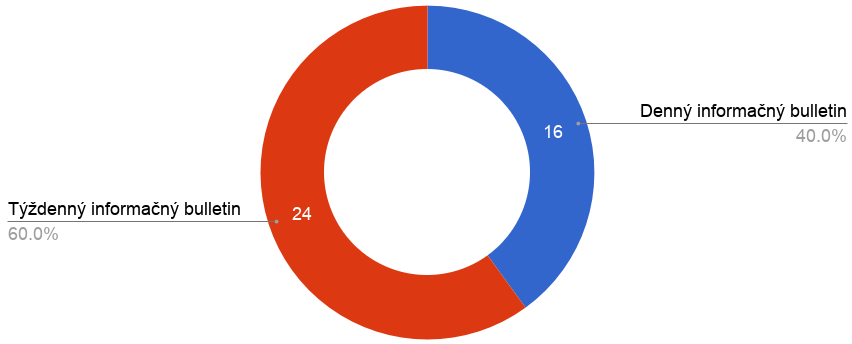
\includegraphics[scale=0.48]{subscriber-doughnut}
\caption{Podiel a počet odoberateľov variant informačného bulletinu.\label{fig:subscriber-chart}}\end{center}
\end{figure}

Systém StackLetter sme propagovali všetkými nami dostupnými spôsobmi: prostredníctvom portálu StackApps\footnote{\url{https://stackapps.com}},
ktorý slúži na prezentáciu aplikácií využívajúcich API platformy Stack Exchange, taktiež prostredníctvom komunitných portálov
Reddit\footnote{\url{https://www.reddit.com/r/stackoverflow/}} a Hacker News\footnote{\url{https://news.ycombinator.com/}},
osobne na fakulte a tiež vo výskumnej skupine \textit{PeWe datalys}\footnote{\url{https://www.pewe.sk/datalys}}.


\section{Metodológia experimentu}
Experiment prebiehal formou A/B testovania. Na rozdiel od štandardného A/B testovania, v ktorom sa používatelia rozdelia
do dvoch alebo viacerých skupín, sme náš test vykonávali na báze striedania použitých metód v časových intervaloch:

\begin{adjustwidth}{1cm}{1cm}
\textbf{1. Kontrolná skupina}\\
V prvej fáze experimentu, od 9. novembra 2017 do 11. marca 2018, sme používateľom generovali informačný bulletin len
prostredníctvom triviálnej metódy odporúčania, ktorá vyberala otázky označené značkami, v ktorých v minulosti používateľ
položil otázku, ponúkol odpoveď alebo okomentoval príspevok. Dáta z tohto časového obdobia slúžili ako kontrolná skupina pre porovnanie
s ostatnými metódami.

Od 12. marca 2018 sme nasadili metódy vytvárania odporúčaní opisované v tejto práci. Metódy generovania informačných bulletinov
sa striedali na týždennej báze.

\textbf{2. Metóda A -- Personalizované odporúčanie}\\
Využívala sa metóda personalizovaného odporúčania opísaná v kapitole~\ref{impl:pers-method}, pričom sa aplikovala
metóda pre zabezpečenie aktuálnosti odporúčaného obsahu. V tomto prípade sa nevykonávala žiadna diverzifikácia odporúčaní.

\textbf{3. Metóda B -- Personalizované odporúčanie s diverzifikáciou}\\
V tomto prípade sa zostavovali personalizované informačné bulletiny s využitím diverzifikačnej metódy tématického
vzorkovania, ako aj metódy pre zabezpečenie aktuálnosti odporúčaného obsahu.
\end{adjustwidth}

A/B testovanie formou striedania metód nám umožnilo vyhnúť sa problému s nerovnomerne rozloženými používateľmi v jednotlivých
skupinách z pohľadu ich aktivity, a tiež nespôsobilo problém pri postupne sa vyvíjajúcom počte používateľov.
Naopak ako potenciálny problém, s~ktorým treba pri takomto riešení počítať, sa ukázalo prirodzené postupné znižovanie
záujmu a~aktivity používateľov počas trvania experimentu.


\section{Metriky hodnotenia výsledkov}

Pre overovanie výsledkov experimentov sme využili nasledovné metriky:

\textbf{Precision@N}\\
Presnosť (angl.~\emph{Precision}), alebo tiež \textit{pozitívna predikčná hodnota} je metrika reprezentujúca pomer relevantných
dokumentov z celkového zoznamu. Štandardne sa presnosť počíta ako pomer z celého zoznamu dokumentov, no v oblasti
odporúčania a vyhľadávania informácií je často vhodnejšou odvodená metrika \textit{Precision@N}, ktorá určuje, aká časť
z prvých N dokumentov v~zozname odporúčaní je pre používateľa relevantná.
$$\mbox{Precision@N}=\frac{|\{\mbox{relevantne otazky v top-N}\}\cap\{\mbox{top-N odporucenych otazok}\}|}
{|\{\mbox{top-N odporucenych otazok}\}|}$$

\textbf{DCG}\\
\textit{Discounted Cumulative Gain} je metrika kvality ohodnocovania často používaná na meranie efektívnosti
odporúčania. DCG meria užitočnosť dokumentov na základe ich pozície vo výslednom zozname. Užitočnosť dokumentov sa akumuluje
od konca zoznamu, pričom najvyššiu užitočnosť majú dokumenty na začiatku zoznamu~\cite{Jrvelin2002}.

DCG položky na pozícii $p$ v zozname odporúčaní je definované ako:

$$\mathrm{DCG_{p}} = \sum_{i=1}^{p} \frac{ 2^{rel_{i}} - 1 }{ \log_{2}(i+1)}$$
\begin{adjustwidth}{1cm}{1cm}
$rel_i$ -- relevancia $i$-tej položky v zozname odporúčaní.\\
\end{adjustwidth}

\textbf{CTR a používateľská aktivita}\\
Miera preklikov (angl.~\emph{Click-through Rate}) je metrika často využívaná v spojitosti s informačnými bulletinmi.
Táto metrika vyjadruje počet úspešných kliknutí na odkaz v informačnom bulletine. V našom experimente sme za úspešné
považovali kliknutia na samotné položky alebo poskytnutie pozitívnej spätnej väzby na položku.

Okrem miery úspešných preklikov sme využili aj odvodenú metriku používateľskej aktivity, ktorá vyjadruje celkový počet
kliknutí na akékoľvek odkazy v informačnom bulletine.

\textbf{Predpoklady výsledkov metrík}\\
Na základe našich hypotéz sme predpokladali nárast vo všetkých sledovaných metrikách pri porovnávaní metódy personalizovaného
odporúčania s kontrolnou skupinou. Pri porovnávaní diverzifikovaného odporúčania a personalizovaného odporúčania sme
predpokladali čiastočný pokles metrík relevancie odporúčaní (Precision@N, DCG), no nárast metrík používateľskej aktivity
-- CTR, impresie, konverzie.


\section{Vyhodnotenie výsledkov experimentu}

V realizovanom online nekontrolovanom experimente, ktorý prebiehal od 9. novembra 2017 a v ktorom boli nasadené navrhnuté
metódy od 12. marca 2018, sa celkovo generovali informačné bulletiny pre 40 používateľov. Počas trvania experimentu
sa z odoberania informačného bulletinu odhlásili traja používatelia. Podrobnejšie štatistiky experimentu uvádza tabuľka
\ref{tab:user-act}.

\begin{table}[h]
\centering
\caption{Štatistika používateľskej aktivity v online experimente.}
\label{tab:user-act}
\begin{tabular}{|m{7cm}|>{\raggedleft\arraybackslash}m{2.5cm}|}
\hline
\textbf{Štatistika} & \textbf{Počet}      \\\hline
Odoberatelia                      &   40  \\\hline
Odoslané informačné bulletiny     & 2400  \\\hline
Otvorené informačné bulletiny     &  750\footnotemark  \\\hline
Celkový počet otvorení bulletinov & 1050  \\\hline
Implicitná spätná väzba           &  530  \\\hline
Explicitná spätná väzba           &  960  \\\hline
Explicitná spätná väzba           &  960  \\\hline
Odhlásenia informačného bulletinu &    3  \\\hline
\end{tabular}
\end{table}

\footnotetext{Počet otvorení informačného bulletinu môže byť skreslený, nakoľko viaceré e-mailové klienty blokujú
zobrazenie obrázkov použitých na vyhodnotenie otvorenia e-mailu. Jedná sa tak o spodnú hranicu reálneho počtu.}

\subsection{Aktivita používateľov}

Aktivita používateľov v informačnom bulletine sa ukázala ako problémový faktor nášho experimentu. Veľká časť používateľov
bola totiž aktívna iba počas prvých dní alebo týždňov od registrácie, a ich aktivita postupom času klesala, ako to
naznačuje aj trendová čiara v grafe~\ref{fig:user-act-hist}. Zvolená metodológia striedania metód po týždňoch však tento
problém do značnej miery eliminovala,
vďaka čomu sa nám podarilo získať dostatočné množstvo dát o aktivite používateľov na to, aby sme vyhodnotili úspešnosť
experimentu (viď tabuľka~\ref{tab:user-act}).


\begin{figure}[H]\begin{center}
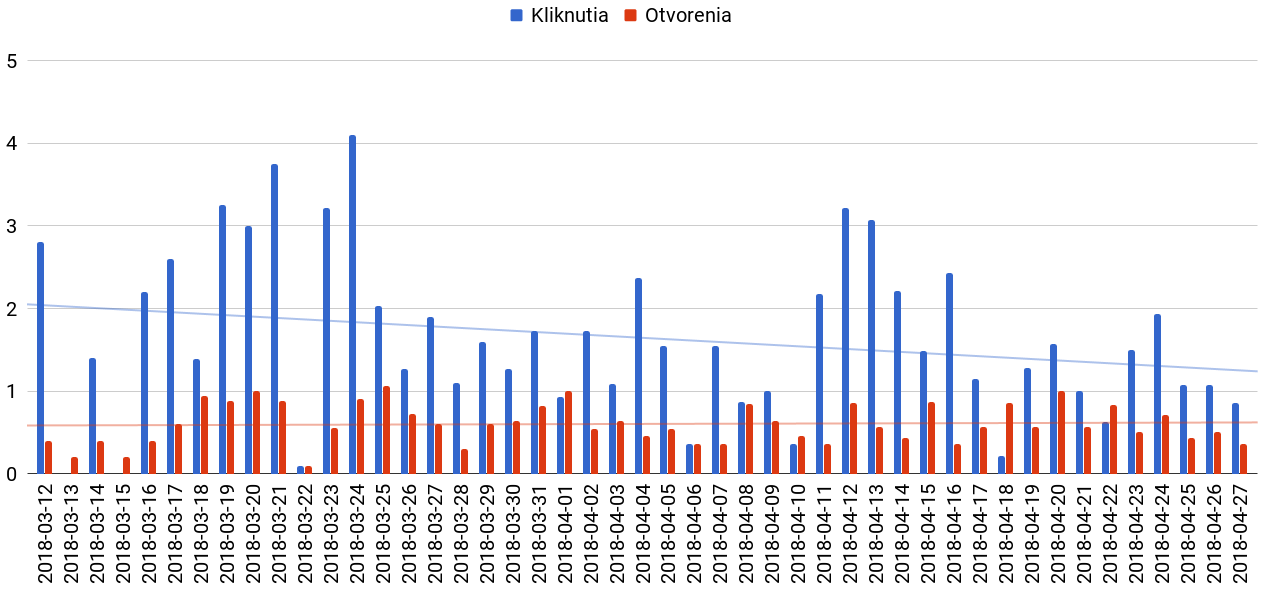
\includegraphics[scale=0.37]{user-activity-hist}
\caption{Priemerná aktivita používateľov v jednotlivých dňoch. \label{fig:user-act-hist}}\end{center}
\end{figure}



\subsection{Vyhodnotenie sledovaných metrík}

\textbf{Presnosť odporúčaní -- Precision@N}\\
Podľa očakávania dosiahla metóda personalizovaného odporúčania výrazne lepšie výsledky pozitívnej predikčnej hodnoty
ako triviálne odporúčanie (viď tabuľka~\ref{tab:pan}), konkrétne približne dvojnásobné. Rovnako podľa očakávania mala
metóda diverzifikácie za dôsledok zníženie presnosti odporúčaní, ktoré však boli aj naďalej výrazne lepšie,
ako v prípade triviálnej metódy.

\begin{table}[H]
\centering
\caption{Priemerné hodnoty Precision@N.}
\label{tab:pan}
\begin{tabular}{|l|c|c|c|c|c|}
\hline
                           & \textbf{N = 1}  & \textbf{N = 2}  & \textbf{N = 3}  & \textbf{N = 4}  & \textbf{N = 5}  \\ \hline
\textbf{Kontrolná skupina} & 0.0266          & 0.0235          & 0.0233          & 0.0232          & 0.0230          \\ \hline
\textbf{Metóda A}          & \textbf{0.0546} & \textbf{0.0506} & \textbf{0.0485} & \textbf{0.0449} & \textbf{0.0473} \\ \hline
\textbf{Metóda B}          & 0.0361          & 0.0356          & 0.0301          & 0.0292          & 0.0274          \\ \hline
\end{tabular}
\end{table}


\textbf{Užitočnosť odporúčaní -- DCG}\\
Metriku DCG sme pre triviálnu metódu odporúčania nepočítali, nakoľko táto metóda nepočítala konkrétne hodnoty relevancie
jednotlivých položiek. Dopad diverzifikačnej metódy tématického vzorkovania na celkovú užitočnosť zoznamu odporúčaní sa ukázal
ako zanedbateľný.

\begin{table}[H]
\centering
\caption{Priemerné hodnoty DCG na pozícii $p$.}
\label{tab:dcgn}
\begin{tabular}{|l|c|c|c|c|c|}
\hline
                  & \textbf{p = 1} & \textbf{p = 2} & \textbf{p = 3} & \textbf{p = 4} & \textbf{p = 5} \\ \hline
\textbf{Metóda A} & \textbf{1.02}  & \textbf{1.66}  & \textbf{2.17}  & \textbf{2.61}  & \textbf{3.00}  \\ \hline
\textbf{Metóda B} & 1.01           & 1.65           & 2.16           & 2.60           & 2.98           \\ \hline
\end{tabular}
\end{table}


\textbf{Spokojnosť používateľov -- CTR a používateľská aktivita}\\
Podľa našich predpokladov z hypotézy 1 sa potvrdilo, že zavedenie personalizovaného odporúčania do informačného bulletinu
CQA systému viedlo k zvýšeniu miery jeho používania a aj celkovej používateľskej aktivity. Hodnoty CTR dosiahli v metóde A
(personalizovaný informačný bulletin) takmer 2,5-násobok voči kontrolnej skupine, celková používateľská aktivita narástla
až na takmer 3,5-násobok.

Predpoklady z hypotézy 2, ktorá hovorila o zvýšení používateľskej aktivity po aplikovaní diverzifikácie, sa v našom
experimente nepotvrdili. Používatelia očakávali personalizované odporúčania, a preto akúkoľvek diverzifikáciu vnímali negatívne,
čo sa prejavilo vo zvýšenom množstve záporných hodnotení položiek prostredníctvom explicitnej spätnej väzby.
Napriek tomu metóda B dosiahla o 42\% lepšie výsledky v metrike CTR voči kontrolnej skupine, a 2,7-násobný nárast v celkovej
aktivite, spôsobený prevažne spomínanou explicitnou spätnou väzbou na položky, ktoré používatelia vnímali ako nerelevantné.

Namerané hodnoty týchto metrík sme overili prostredníctvom analýzy rozptylu (ANOVA), ktorá potvrdila, že sú štatisticky
signifikantné.

Výsledky týchto metrík ukazujú, že používatelia, ktorí boli súčasťou nášho online experimentu nevnímajú v prípade
informačných bulletinov uzavretie do \textit{filtračnej bubliny} ako problém, ale naopak ako žiadaný stav.

\begin{table}[H]
\centering
\caption{Priemerné hodnoty CTR a používateľskej aktivity.}
\label{tab:ctr}
\begin{tabular}{|l|c|c|}
\hline
                           & \textbf{CTR}   & \textbf{\begin{tabular}[c]{@{}c@{}}Používateľská\\ aktivita\end{tabular}} \\ \hline
\textbf{Kontrolná skupina} & 0.024          & 0.036           \\ \hline
\textbf{Metóda A}          & \textbf{0.058} & \textbf{0.123}  \\ \hline
\textbf{Metóda B}          & 0.034          & 0.098           \\ \hline \hline
\multicolumn{3}{|c|}{\textbf{ANOVA}}                          \\ \hline
\textbf{F-value}           & 12.69        & 34.14             \\ \hline
\textbf{P-value}           & $3×10^{-6}$  & $2×10^{-15}$      \\ \hline
\end{tabular}
\end{table}


\subsection{Dotazník odoberateľov}

Súčasťou vyhodnotenia bol aj dotazník pre odoberateľov informačného bulletinu. Dotazník od 21. apríla 2018 vyplnilo 27.5\%
odoberateľov. Celkovo boli odoberatelia na základe odpovedí z dotazníku spokojní s ponúkaným obsahom. 63\% z nich si všimlo,
že obsah bol personalizovaný a všetci respondenti považujú personalizáciu obsahu informačných bulletinov za užitočnú a za veľmi
dobrý nápad.

Odoberatelia nevedeli subjektívne posúdiť, či bol pre nich ponúkaný obsah relevantný, väčšina z nich zvolila prostrednú možnosť.
55\% respondentov označilo subjektívne svoju aktivitu za podpriemernú, 45\% z nich sa označilo za mierne aktívnejších.

Výsledky z dotazníku samozrejme môžu byť do určitej miery skreslené, keďže v nich respondenti prezentujú svoje subjektívne
postoje. Zároveň predpokladáme, že skupina neaktívnych odoberateľov dotazník nevyplnila vôbec, preto ich postoje nemusia
byť adekvátne zastúpené. Podrobné výsledky dotazníku sú priložené v dokumente v prílohe~\ref{appendix:survey}.


\section{Diskusia}

Overenie našich hypotéz a navrhnutých metód prostredníctvom online nekontrolovaného experimentu je v oblasti odporúčania
v CQA systémoch pomerne unikátnym javom, keďže realizácia takéhoto experimentu je pomerne náročná nie len časovo,
ale aj z pohľadu možnosti kontrolovať priebeh a výsledky experimentu. Napriek tomu tento experiment považujeme za úspešný,
nakoľko priniesol pomerne zaujímavé výsledky.

Experiment potvrdil, že používatelia majú záujem o personalizované odporúčanie aj v informačných bulletinoch CQA systémov,
čo sa zároveň prejavuje na ich zvýšenej aktivite a záujme o informačný bulletin. Celkovo má personalizácia pozitívny vplyv
na všetky sledované metriky.

Ako nečakaný výsledok sa ukázalo, že fenomén tzv. filtračnej bubliny, ktorý sa pri výskume často považuje za problém, tak
používatelia nevnímajú, a naopak ho očakávajú. To sa v experimente prejavilo najmä znížením celkovej aktivity používateľov
v informačných bulletinoch využívajúcich diverzifikačnú metódu, ako aj zvýšením negatívnej spätnej väzby. Napriek tomu
aj diverzifikované informačné bulletiny vnímajú výrazne pozitívnejšie ako informačné bulletiny bez personalizácie.

V súvislosti s aktivitou používateľov sa prejavilo aj negatívne vnímanie informačných bulletinov ako spamu,
čo spôsobovalo problém pri získavaní nových používateľov a udržiavaní aktivity existujúcich odoberateľov.

Treba tiež pripustiť možné obmedzenia vykonávaného experimentu, najmä trochu nižší počet používateľov a tiež relatívne
nízky podiel aktívnych používateľov. Tieto obmedzenia však vyvažuje fakt, že sa jednalo o online nekontrolovaný experiment,
ktorý je výrazne realistickejší ako prípadné offline simulované experimenty, ktoré sú v tejto doméne najčastiejšie.
